% fixture: tikz/tree-edges-pdftex
% oracle: pdflatex
% tier: T3
% engine: document
% specials: compare
% covers: TikZ trees' edges (edge from parent with options and with labels placed on it, the edge from parent style, edge from parent path with the parent's and the child's node and anchor, parent anchor, child anchor and border, every child and every child node, what follows a child's node drawn before its edge)
\documentclass{article}
\usepackage{tikz}
\pagestyle{empty}
\begin{document}
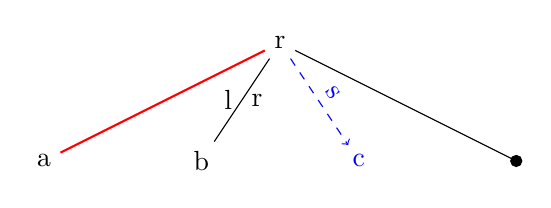
\begin{tikzpicture}[sibling distance=2cm]
  \node {r}
    child { node {a} edge from parent[red, thick] }
    child { node {b} edge from parent node[left] {l} node[right] {r} }
    child[blue] { node {c} edge from parent[dashed, ->] node[above, sloped] {s} }
    child { [fill] circle (2pt) };
\end{tikzpicture}

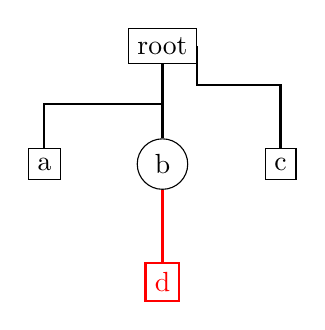
\begin{tikzpicture}[parent anchor=south, child anchor=north, every child node/.style={draw},
  edge from parent/.style={draw, thick},
  edge from parent path={(\tikzparentnode\tikzparentanchor) -- ++(0,-5mm) -| (\tikzchildnode\tikzchildanchor)}]
  \node[draw] {root}
    child { node {a} }
    child[every child/.style={red}] { node[circle] {b} child { node {d} } }
    child[child anchor=west] { node {c} edge from parent[parent anchor=east, child anchor=border] };
\end{tikzpicture}
\end{document}
